\section{Data and Summary Statistics:}

Table XXXXX presents descriptive statistics for the main variables included in the model. Our dependent variable, the logarithmic per capita household income, shows an upward trend in mean values, peaking at 5.749 in 2019 before slightly declining in 2020 and then modestly recovering in 2021. The standard deviation, ranging from 0.883 to 0.836, reflects moderate dispersion relative to the mean based on the coefficient of variation across every period. This level of variability suggests that predictions using this variable as dependent will have a reasonable level of accuracy, providing robust yet not extremely precise forecasts. Its lagged values exhibit similar patterns in both mean and standard deviation. The moderate dispersion of these suggests that some degree of temporal autocorrelation exists, meaning the variable's historical values provide useful information for forecasting.
Regarding household characteristics, the average number of children per household has shown a declining trend, from 1.006 in 2017 to 0.965 in 2021, with an unusual increase to 1.012 in 2020, possibly due to the COVID-19 pandemic. The relatively high dispersion, as indicated by standard deviations ranging from 1.319 to 1.267, indicates significant variability in family sizes across the sample, which demonstrates how family planning preferences vary across different socioeconomic levels.
The education variables — incomplete primary ("prii"), incomplete secondary ("seci"), complete secondary ("secc"), incomplete higher education ("supi"), and complete higher education ("supc") — reveal that a significant proportion of the population has education levels below higher education, revealing potential limitations in workforce skills development. These statistics highlight the challenges faced by the education system in increasing educational attainment beyond the secondary level, which may constrain social mobility and limit economic opportunities, ultimately impacting household income.
The sample also has a mean age of around 52 years across all periods, with a high standard deviation of around 15.5 years, reflecting substantial age dispersion. The proportion of males remains relatively constant at around 0.71, with a moderate standard deviation of approximately 0.44.
Lastly, the informal employment rate demonstrates a steady mean value of 0.58 across the years, with a standard deviation close to 0.49, indicating moderate variability in informal employment status. This high rate of informal employment is often associated with lower wages, reduced job security, and limited access to social protection, which may deeply explain household income patterns. Altogether, these variables provide valuable economic information with appropriate levels of dispersion, offering predictive power for the per capita household income.


% Insert enaho table here:

Table XXXXX presents descriptive statistics for predictors included in the forecasting model which were derived from geospatial and environmental data. These contain information on the evolution of precipitation, temperature, and nightlight for the location of every observation.
Starting with the precipitation, the standard deviation has shown variability over the years, beginning at 5.182 in the period 2010-2016, increasing to 8.618 in 2019, then decreasing to 6.918 in 2020, and 6.541 in 2021. These fluctuations suggest notable differences in weather patterns, which could influence agricultural productivity and household income in regions heavily dependent on agriculture, as is common in various regions of Peru.
Regarding temperatures, the standard deviation for maximum temperature is relatively stable, fluctuating between 0.276 and 0.272. Minimum temperature shows similar stability, fluctuating between 0.318 and 0.327. This consistency implies limited fluctuation in extreme temperatures, which may impact energy consumption patterns, agricultural output, and health-related expenditures, indirectly affecting household income.
Finally, regarding the nightlight, this data provides an indirect measure of economic activity and infrastructure development in the observation’s location. The maximum nightlight variable shows significant variability, with standard deviations ranging from 63.068 in 2018 to 91.132 in 2020. This suggests variations in economic development levels, potentially correlating with regional economic disparities. The standard deviation of mean nightlight, ranging from 8.137 to 17.149, indicates that some areas experience significant variations in economic activity. The range of nightlight data (up to 90.567) reinforces these disparities, emphasizing differences in infrastructure and economic development.

% Insert geo and nightlight table here:

Table XXXXXX presents descriptive statistics for predictors included in the forecasting model, derived from administrative data. These statistics detail the evolution of various crime indicators, the cargo industry, general industry labor metrics, public revenue, and public expenditure. Analyzing crime variables reveals significant trends and dynamics within different categories. Economic Commercial Offenses exhibited the most significant reduction, with the mean decreasing from 0.472 to 0.409. In contrast, Theft Robbery Related Crimes saw the largest increase, with the mean growing from 720.964 to 1662.403. Fraud Financial Crimes and Sexual Offenses also experienced notable increases, with their means rising to 113.783 and 115.548, respectively. Intellectual Property violations showed the smallest change in mean, modestly increasing from 0.288 to 0.735. Regarding variability, Public Order Political Crimes initially had the highest standard deviation at 921.22, which has substantially narrowed over time, suggesting a stabilization in the frequency, and reporting of these offenses.
Analyzing cargo vehicle-related variables provides key insights into economic activity at each observation's location. The total number of vehicles (vehicles_tot) demonstrated a mean increase from 7.152 to 18.689 over the years, indicating overall growth in fleet size. Vehicle age metrics (fab_5y_p, fab_10y_p, fab_20y_p, fab_30y_p) offer insights into fleet modernization trends. The mean percentage of vehicles under 5 years (fab_5y_p) slightly decreased over time, suggesting a slower fleet renewal rate, with similar trends observed in the 10, 20, and 30-year metrics. The standard deviations in these age categories highlight variability in fleet renewal practices. The mean percentage of public sector vehicles has increased from 0.816 to 0.884. Payload capacity (payload_m) also varied significantly, with mean values rising from 11,150.79 to 14,429.07, suggesting an improvement in transport efficiency. Vehicle specifications such as dry weight and gross weight showed fluctuating means, with dry weight increasing from 5760.224 to 6504.72, and gross weight from 8.002 to 8.578. The high level of standard deviations for these variables reflects considerable diversity in vehicle types, modernity, and capacities. This variability is crucial for forecasting household per capita income as it affects economic activity and job availability in regions heavily reliant on the cargo industry.
Analyzing labor market variables provides insights into the dynamics between supply and demand in the industry. The number of companies (companies) showed an upward trend, increasing from an average of 1,264 to 1,614, reflecting a rise in labor demand. Concurrently, the total number of workers (workers_tot) also increased from about 14,011 to 18,239, indicating a growth in labor supply. Gender representation shifted slightly, with female participation (workers_sex_f_perc) increasing from 0.279 to 0.300, while male participation (workers_sex_m_perc) decreased from 0.640 to 0.626. The workforce structure saw a decrease in executives (workers_type_exe_perc) from 0.031 to 0.025, and general workers (workers_type_wor_perc) from 0.297 to 0.270, while employed staff (workers_type_emp_perc) rose from 0.648 to 0.662. The average salary (salaries_mean) increased from 1,612 to 1,873, aligning with sectorial growth. The standard deviations across these metrics reveal significant diversity in company sizes, workforce compositions, and compensation policies, highlighting varied industry practices.
We proceed to analyze public revenue variables. Revenues from the mining sector (canon) have experienced a significant mean increase from 1,615,520 to 2,005,037, reflecting heightened mining activity. The foncomun, a pool of funds redistributed among municipalities, exhibits growth in mean values from 1,003,377 to 1,874,736. Municipal taxes (Impuestos municipales) have shown an upward trend in mean revenue from 1,004,646 to 1,809,327, which indicates stronger local tax collection efforts or economic growth that enhances the tax base. Finally, directly collected revenues (recursos_directamente_recaudados) have seen mean values rise from 1,031,412 to 1,649,157. Despite these increases, the variability in these revenue variables, as suggested by their standard deviations, points to disparities in economic activity, fiscal management proficiency, and reliance on sectors like mining across different regions.
Finally, when analyzing public expenditure variables, we observe significant changes in their means and variability, which are crucial for understanding government spending priorities and their stability. Public health expenditure demonstrated the highest increase in mean values, rising from 54,529 to 110,229, indicating a growing focus on healthcare infrastructure. In terms of variability, transport expenditure displayed the greatest increase, with standard deviations expanding from 2,919,155 to 21,213,497, suggesting fluctuating investments possibly driven by large-scale projects or inconsistent funding. Conversely, urban development showed the most stable spending patterns, with a slight decrease in variability from 1,495,590 to 1,379,319. These dynamics in public spending directly impact the forecasting of household per capita income, particularly as they relate to the provision of public services that can significantly alleviate household expenditures, thus enabling families to redirect or save a portion of their income for other uses.


% Insert admin data table here:



\begin{figure}[H]
    \caption{Correlation of log(Income) with Lagged Conglomerate Log Income}
    \centering
         \centering
         \begin{subfigure}[b]{0.47\textwidth}
             \centering
             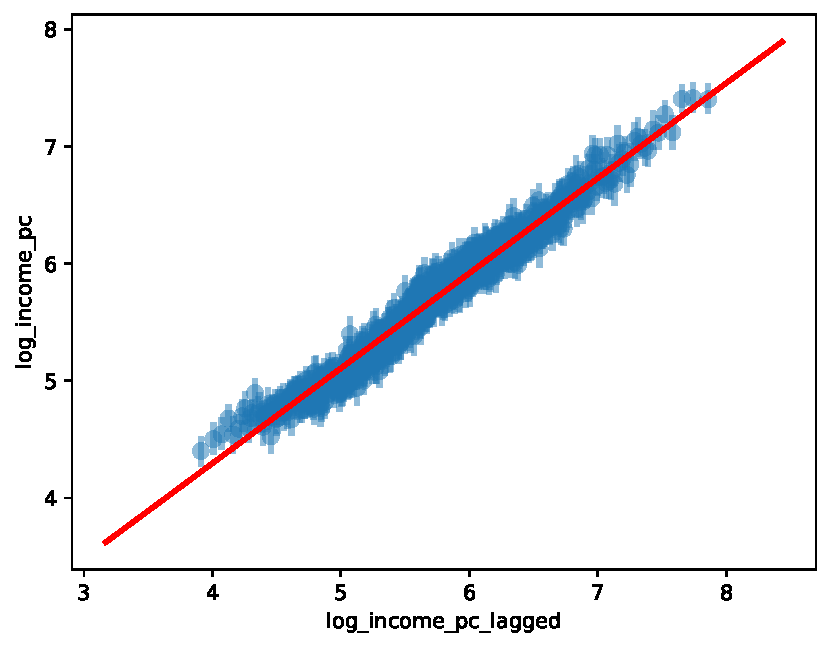
\includegraphics[width=\textwidth]{../figures/figA_income_vs_lagged_income_log_log_scatterplot.pdf}
             \caption{Lag: t-1}
         \end{subfigure}
         \hfill
         \begin{subfigure}[b]{0.47\textwidth}
             \centering
             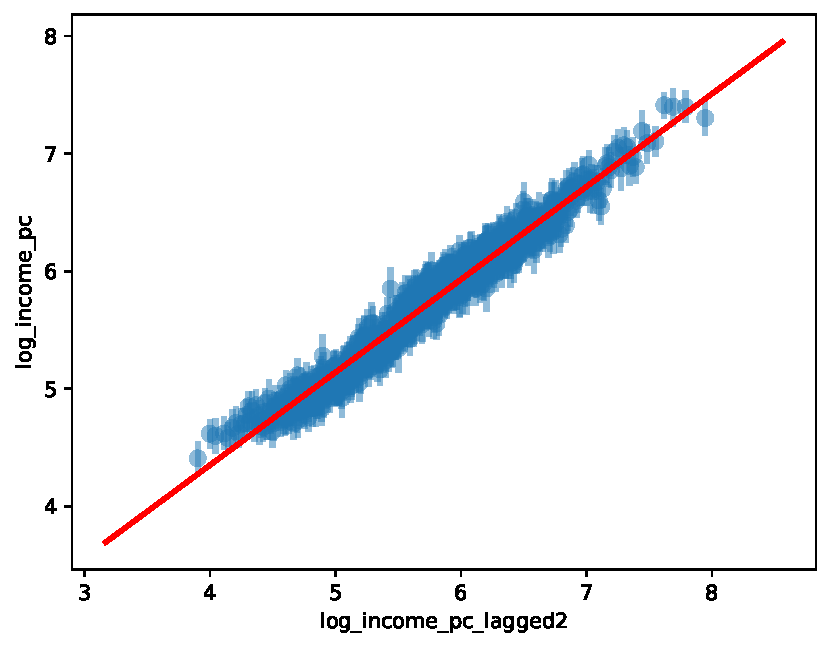
\includegraphics[width=\textwidth]{../figures/figA_income_vs_lagged2_income_log_log_scatterplot.pdf}
             \caption{Lag: t-2}
         \end{subfigure} 
          \hfill
         \begin{subfigure}[b]{0.47\textwidth}
             \centering
             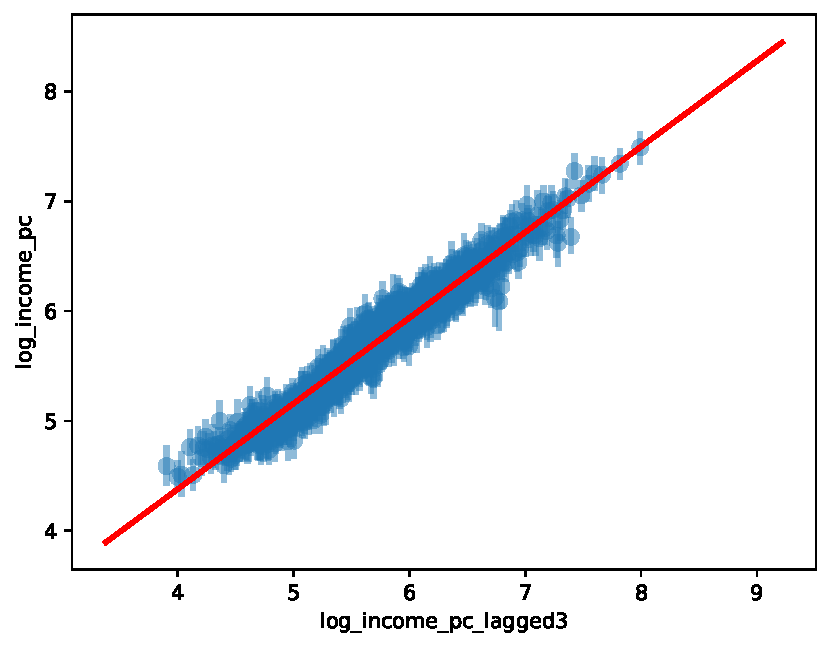
\includegraphics[width=\textwidth]{../figures/figA_income_vs_lagged3_income_log_log_scatterplot.pdf}
             \caption{Lag: t-3}
         \end{subfigure} 
          \hfill
         \begin{subfigure}[b]{0.47\textwidth}
             \centering
             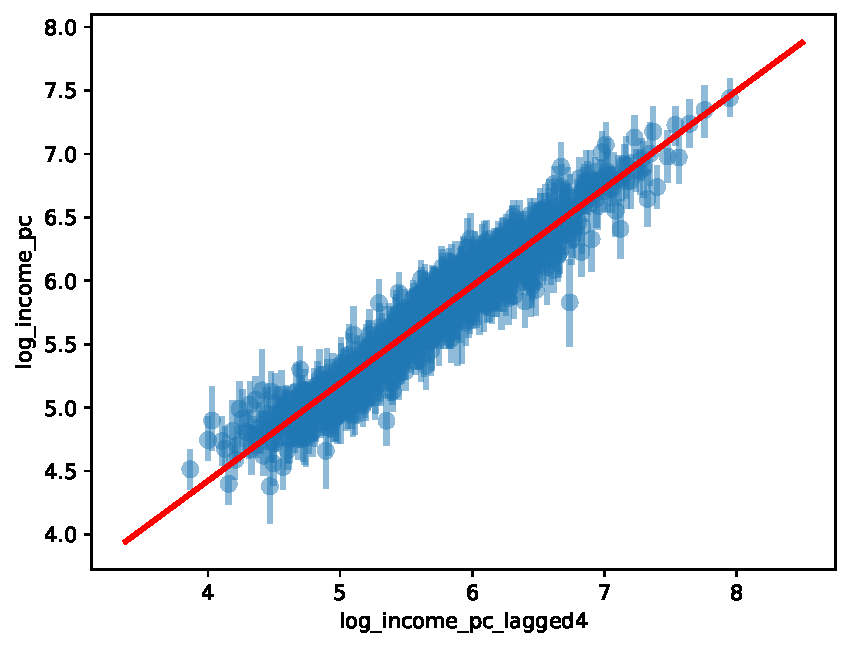
\includegraphics[width=\textwidth]{../figures/figA_income_vs_lagged4_income_log_log_scatterplot.pdf}
             \caption{Lag: t-4}
         \end{subfigure} 
    \subcaption*{Note:} 
    \end{figure}


\begin{figure}[H]
    \centering
    \caption{Distribution for each variable}
    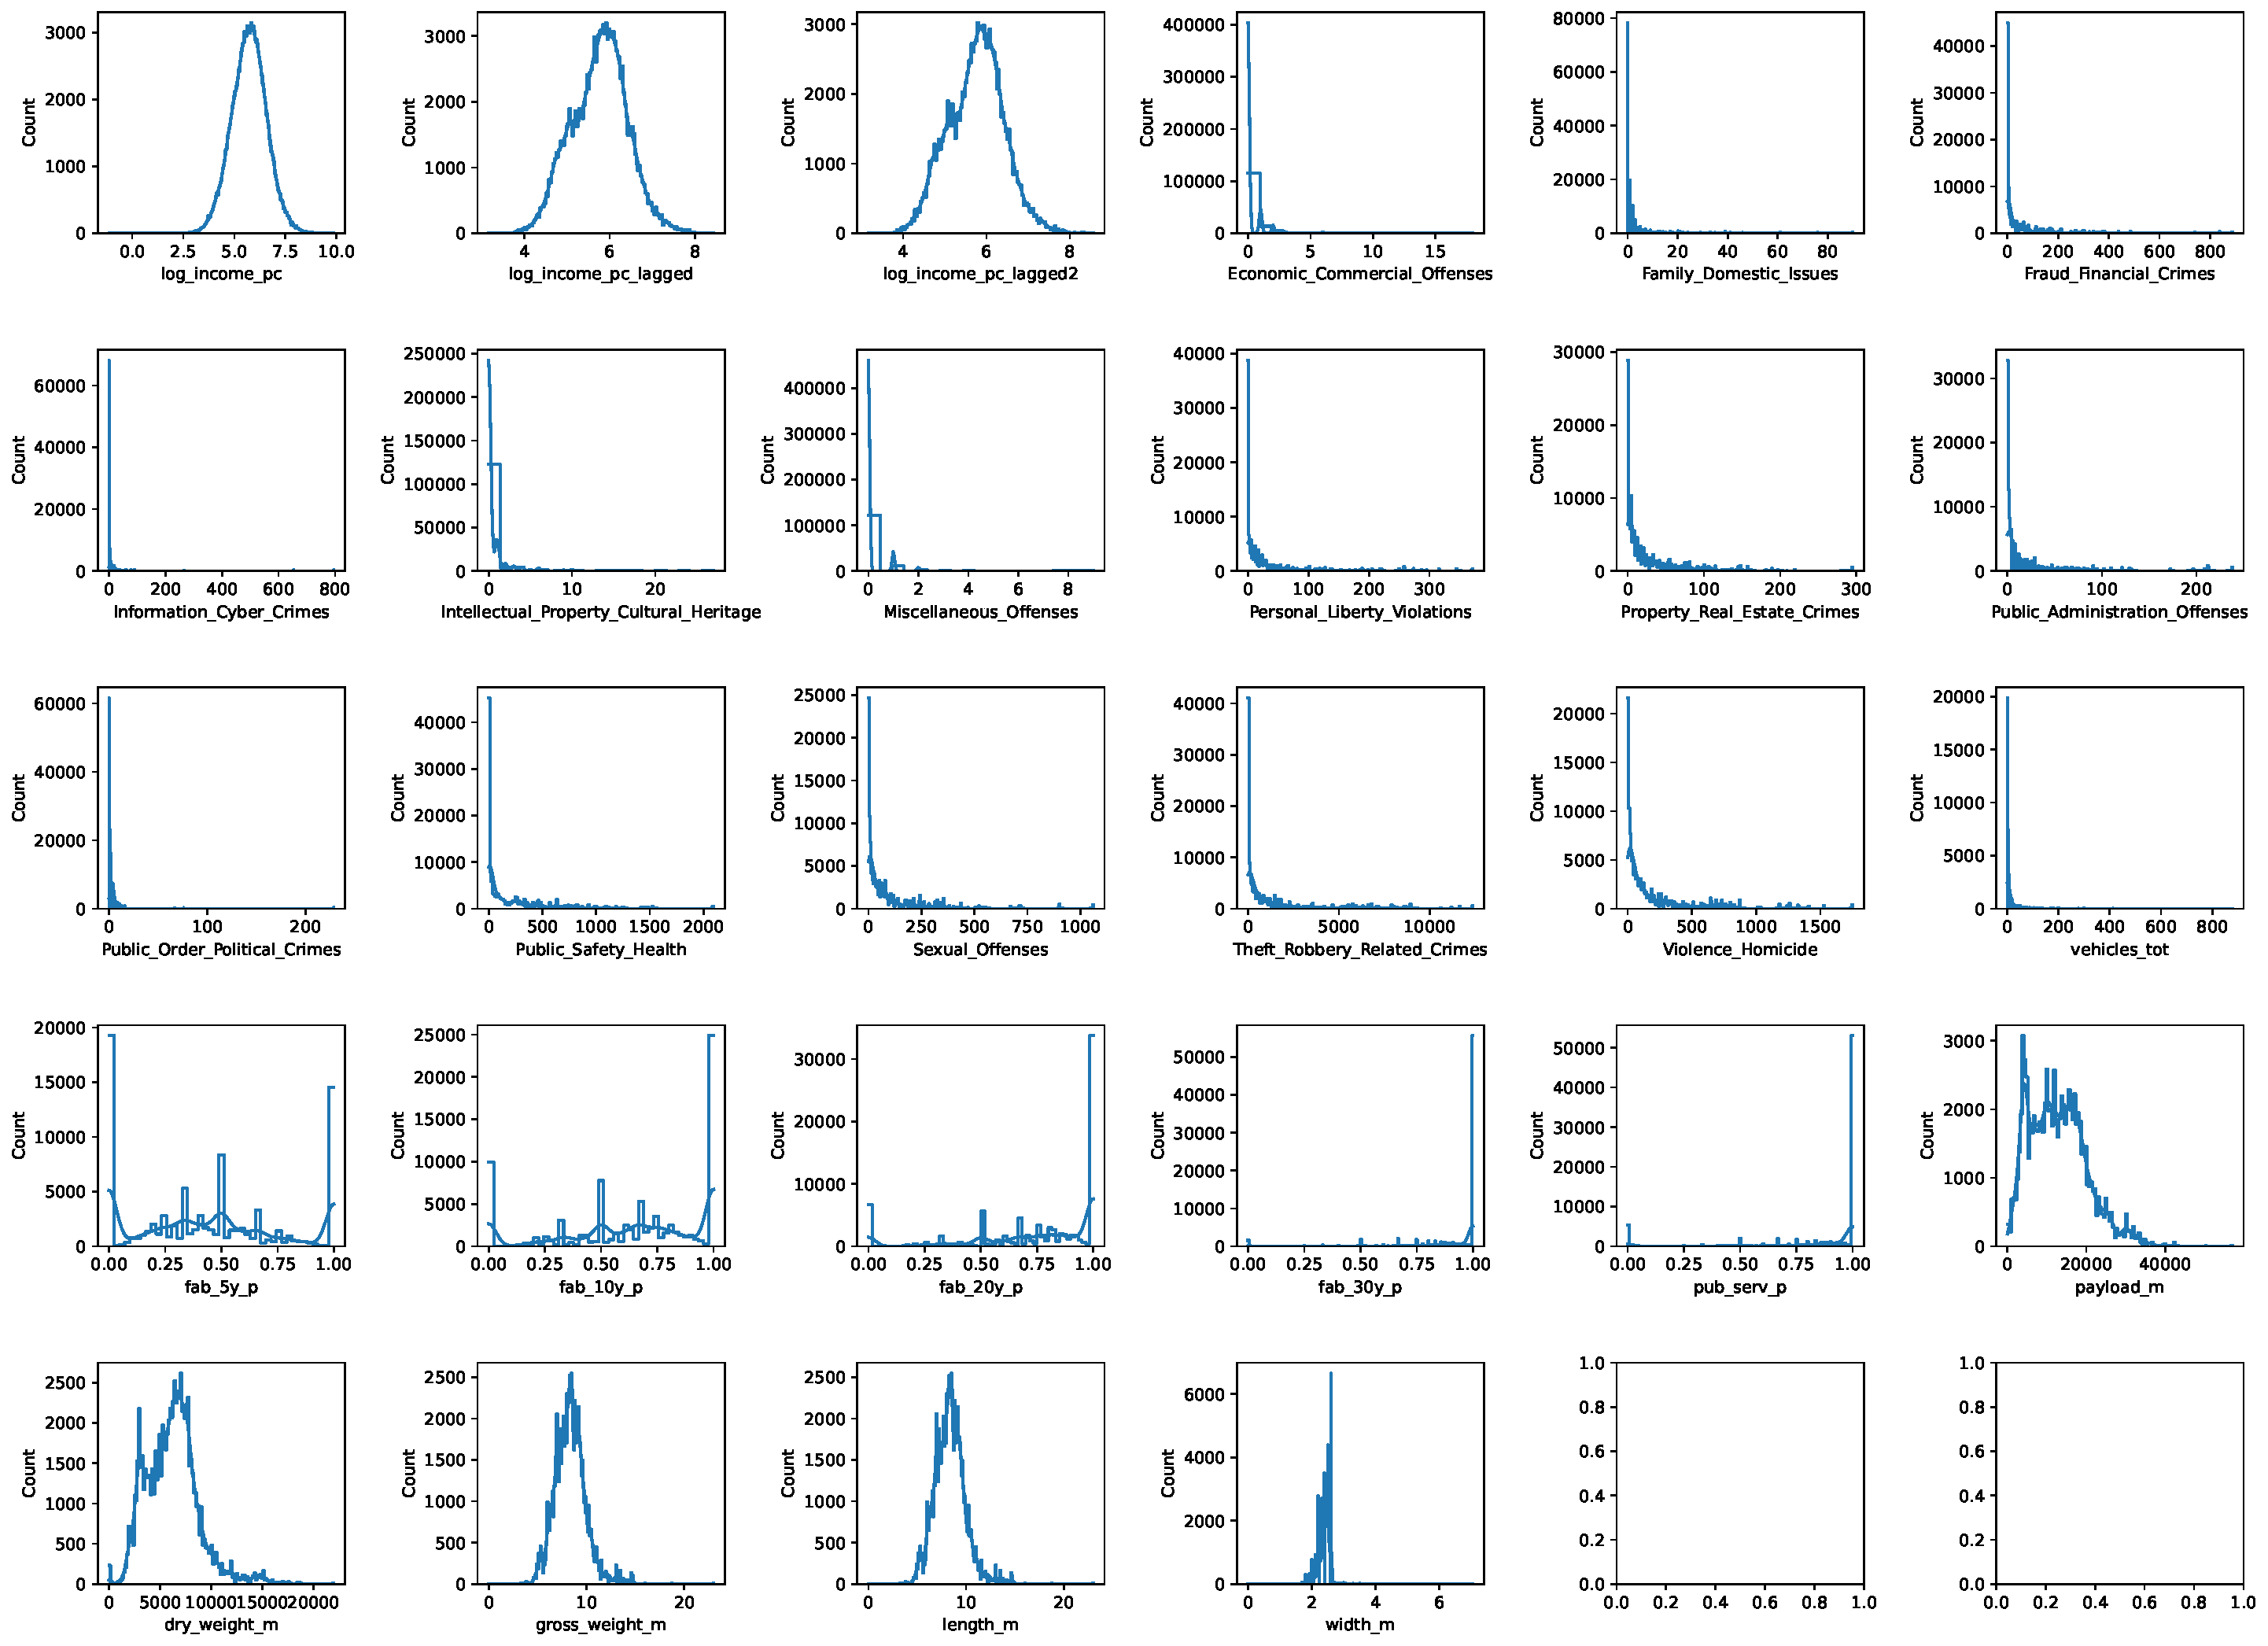
\includegraphics[width=1\textwidth]{../figures/figB_histograms_ml_dataset_variables.pdf}
    \label{fig:enter-label}
\end{figure}


\begin{figure}[H]
    \centering
    \caption{Correlation of log(Income) with variables}
    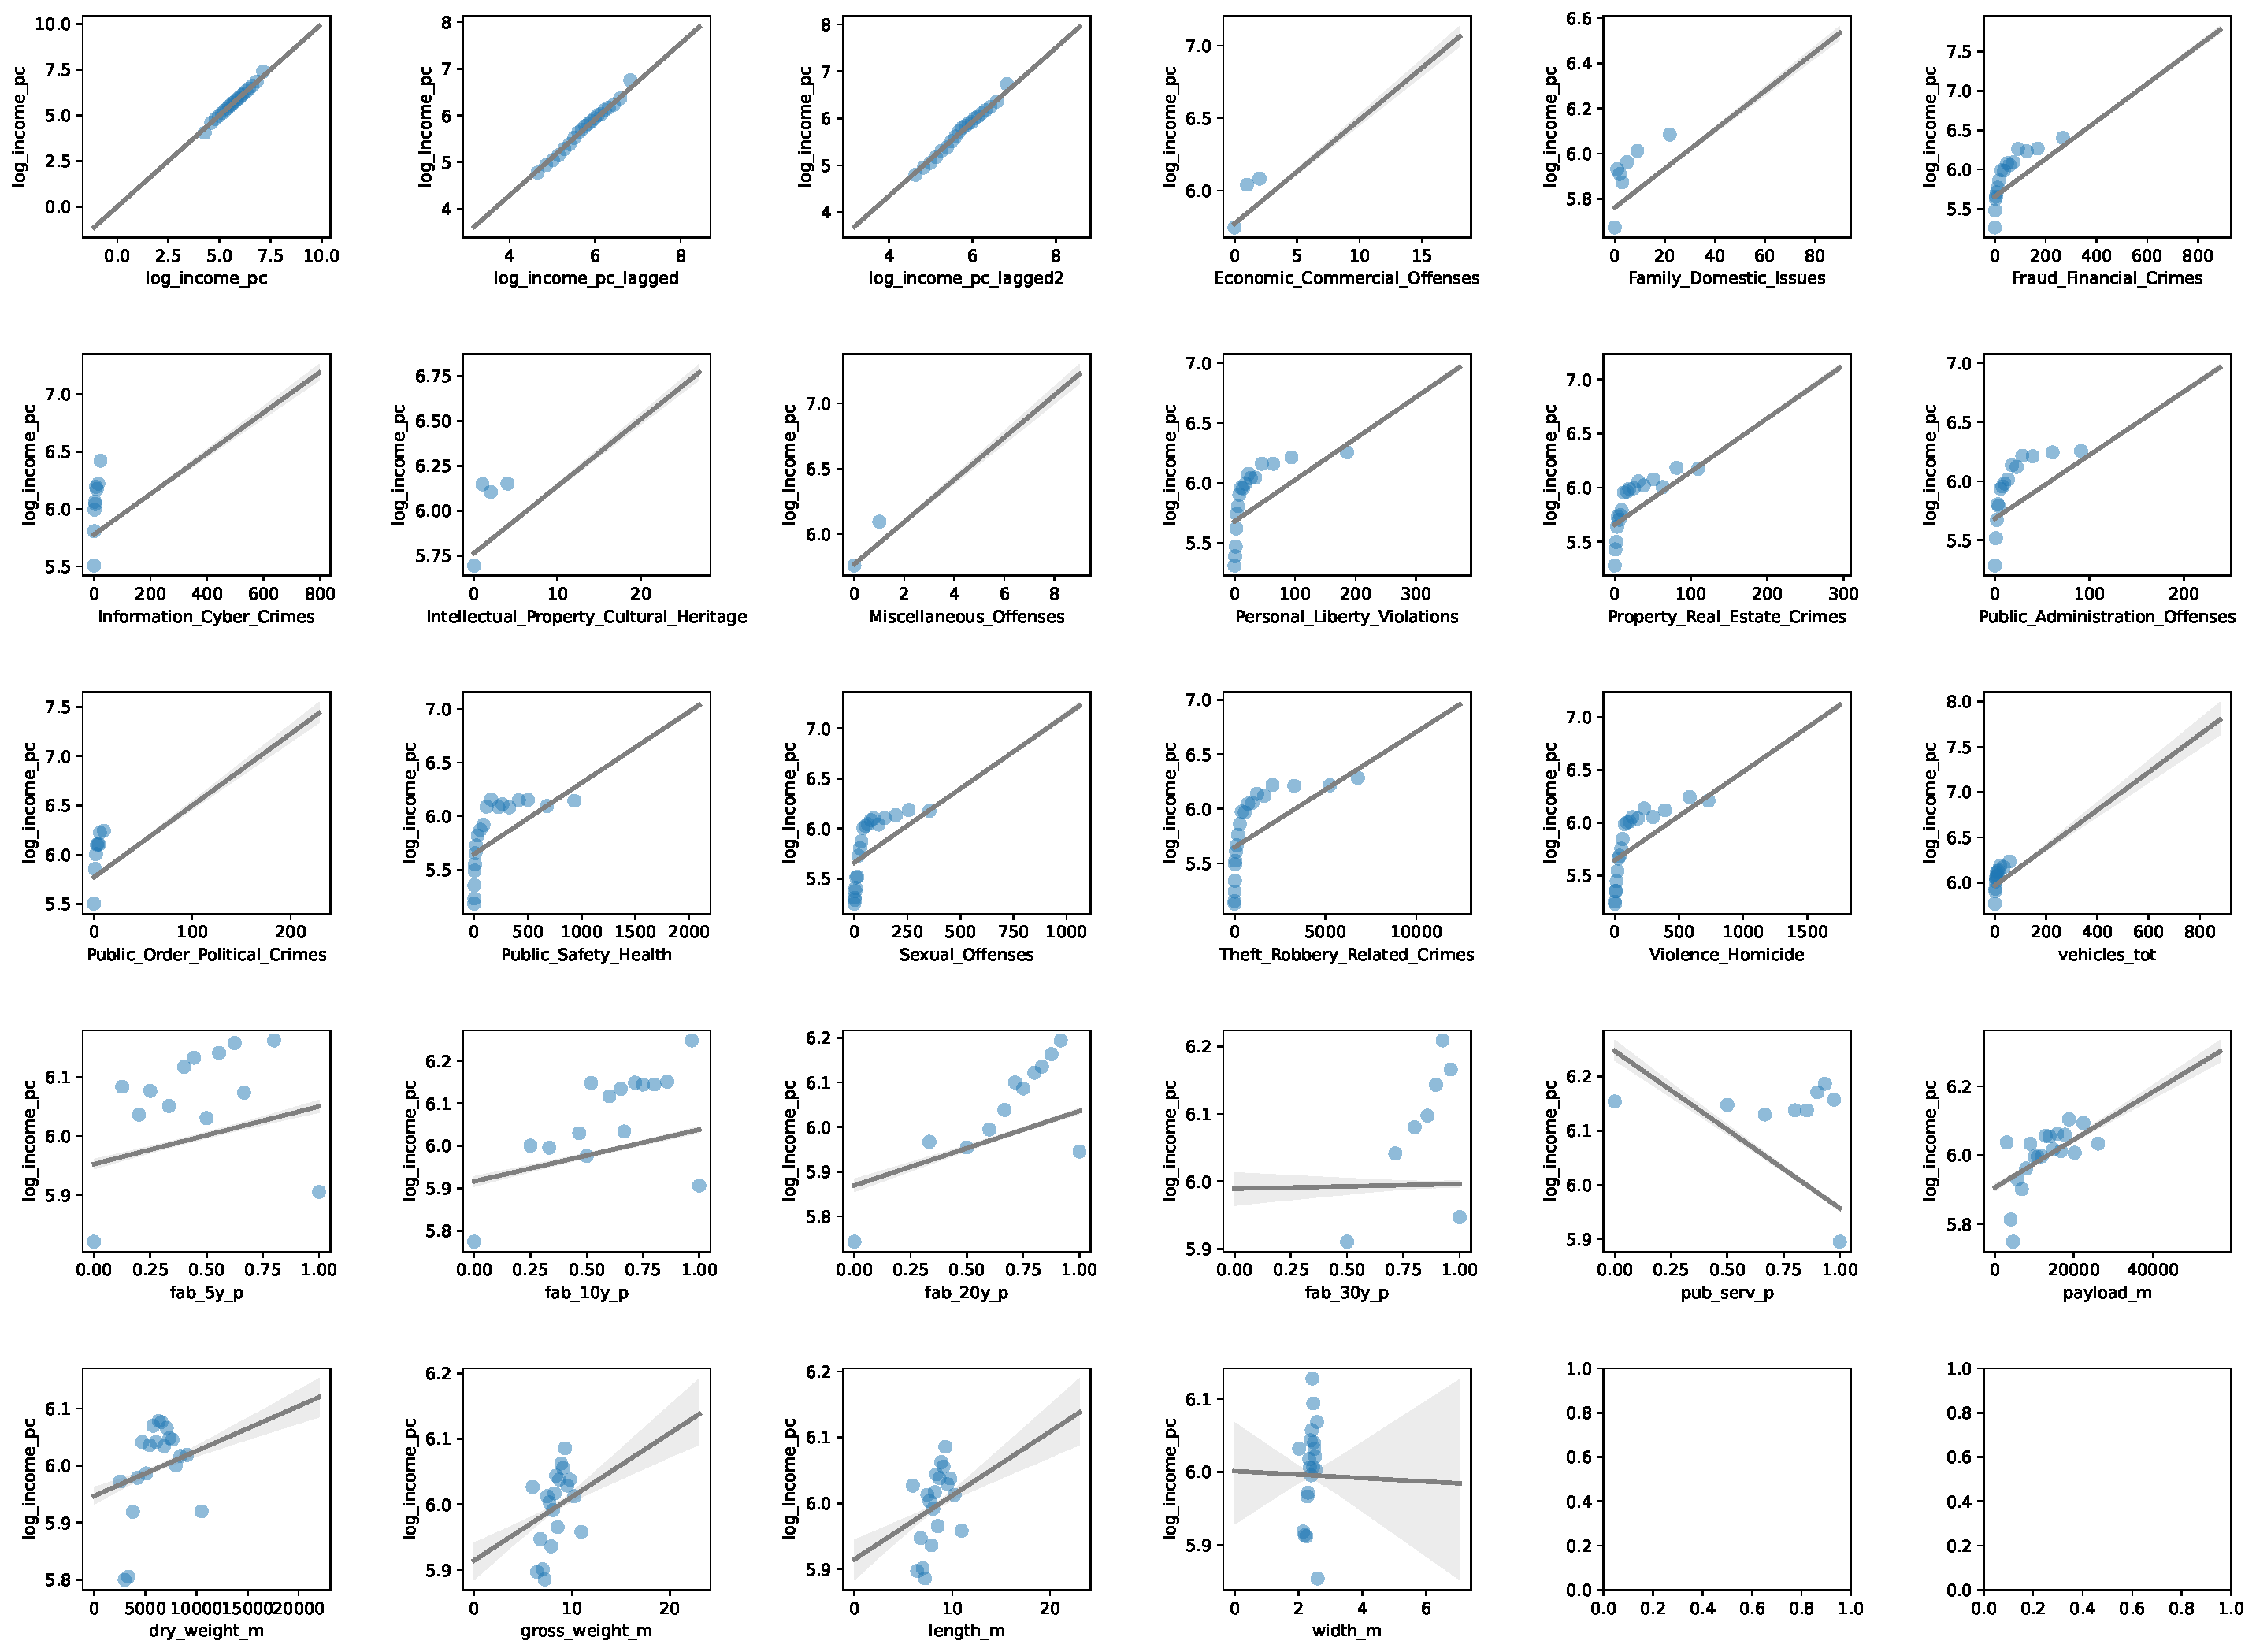
\includegraphics[width=1\textwidth]{../figures/figC_correlation_ml_dataset_variables.pdf}
    \label{fig:enter-label}
\end{figure}


\begin{figure}[H]
    \centering
    \caption{Correlation of log(Income) with Weather Variables}
    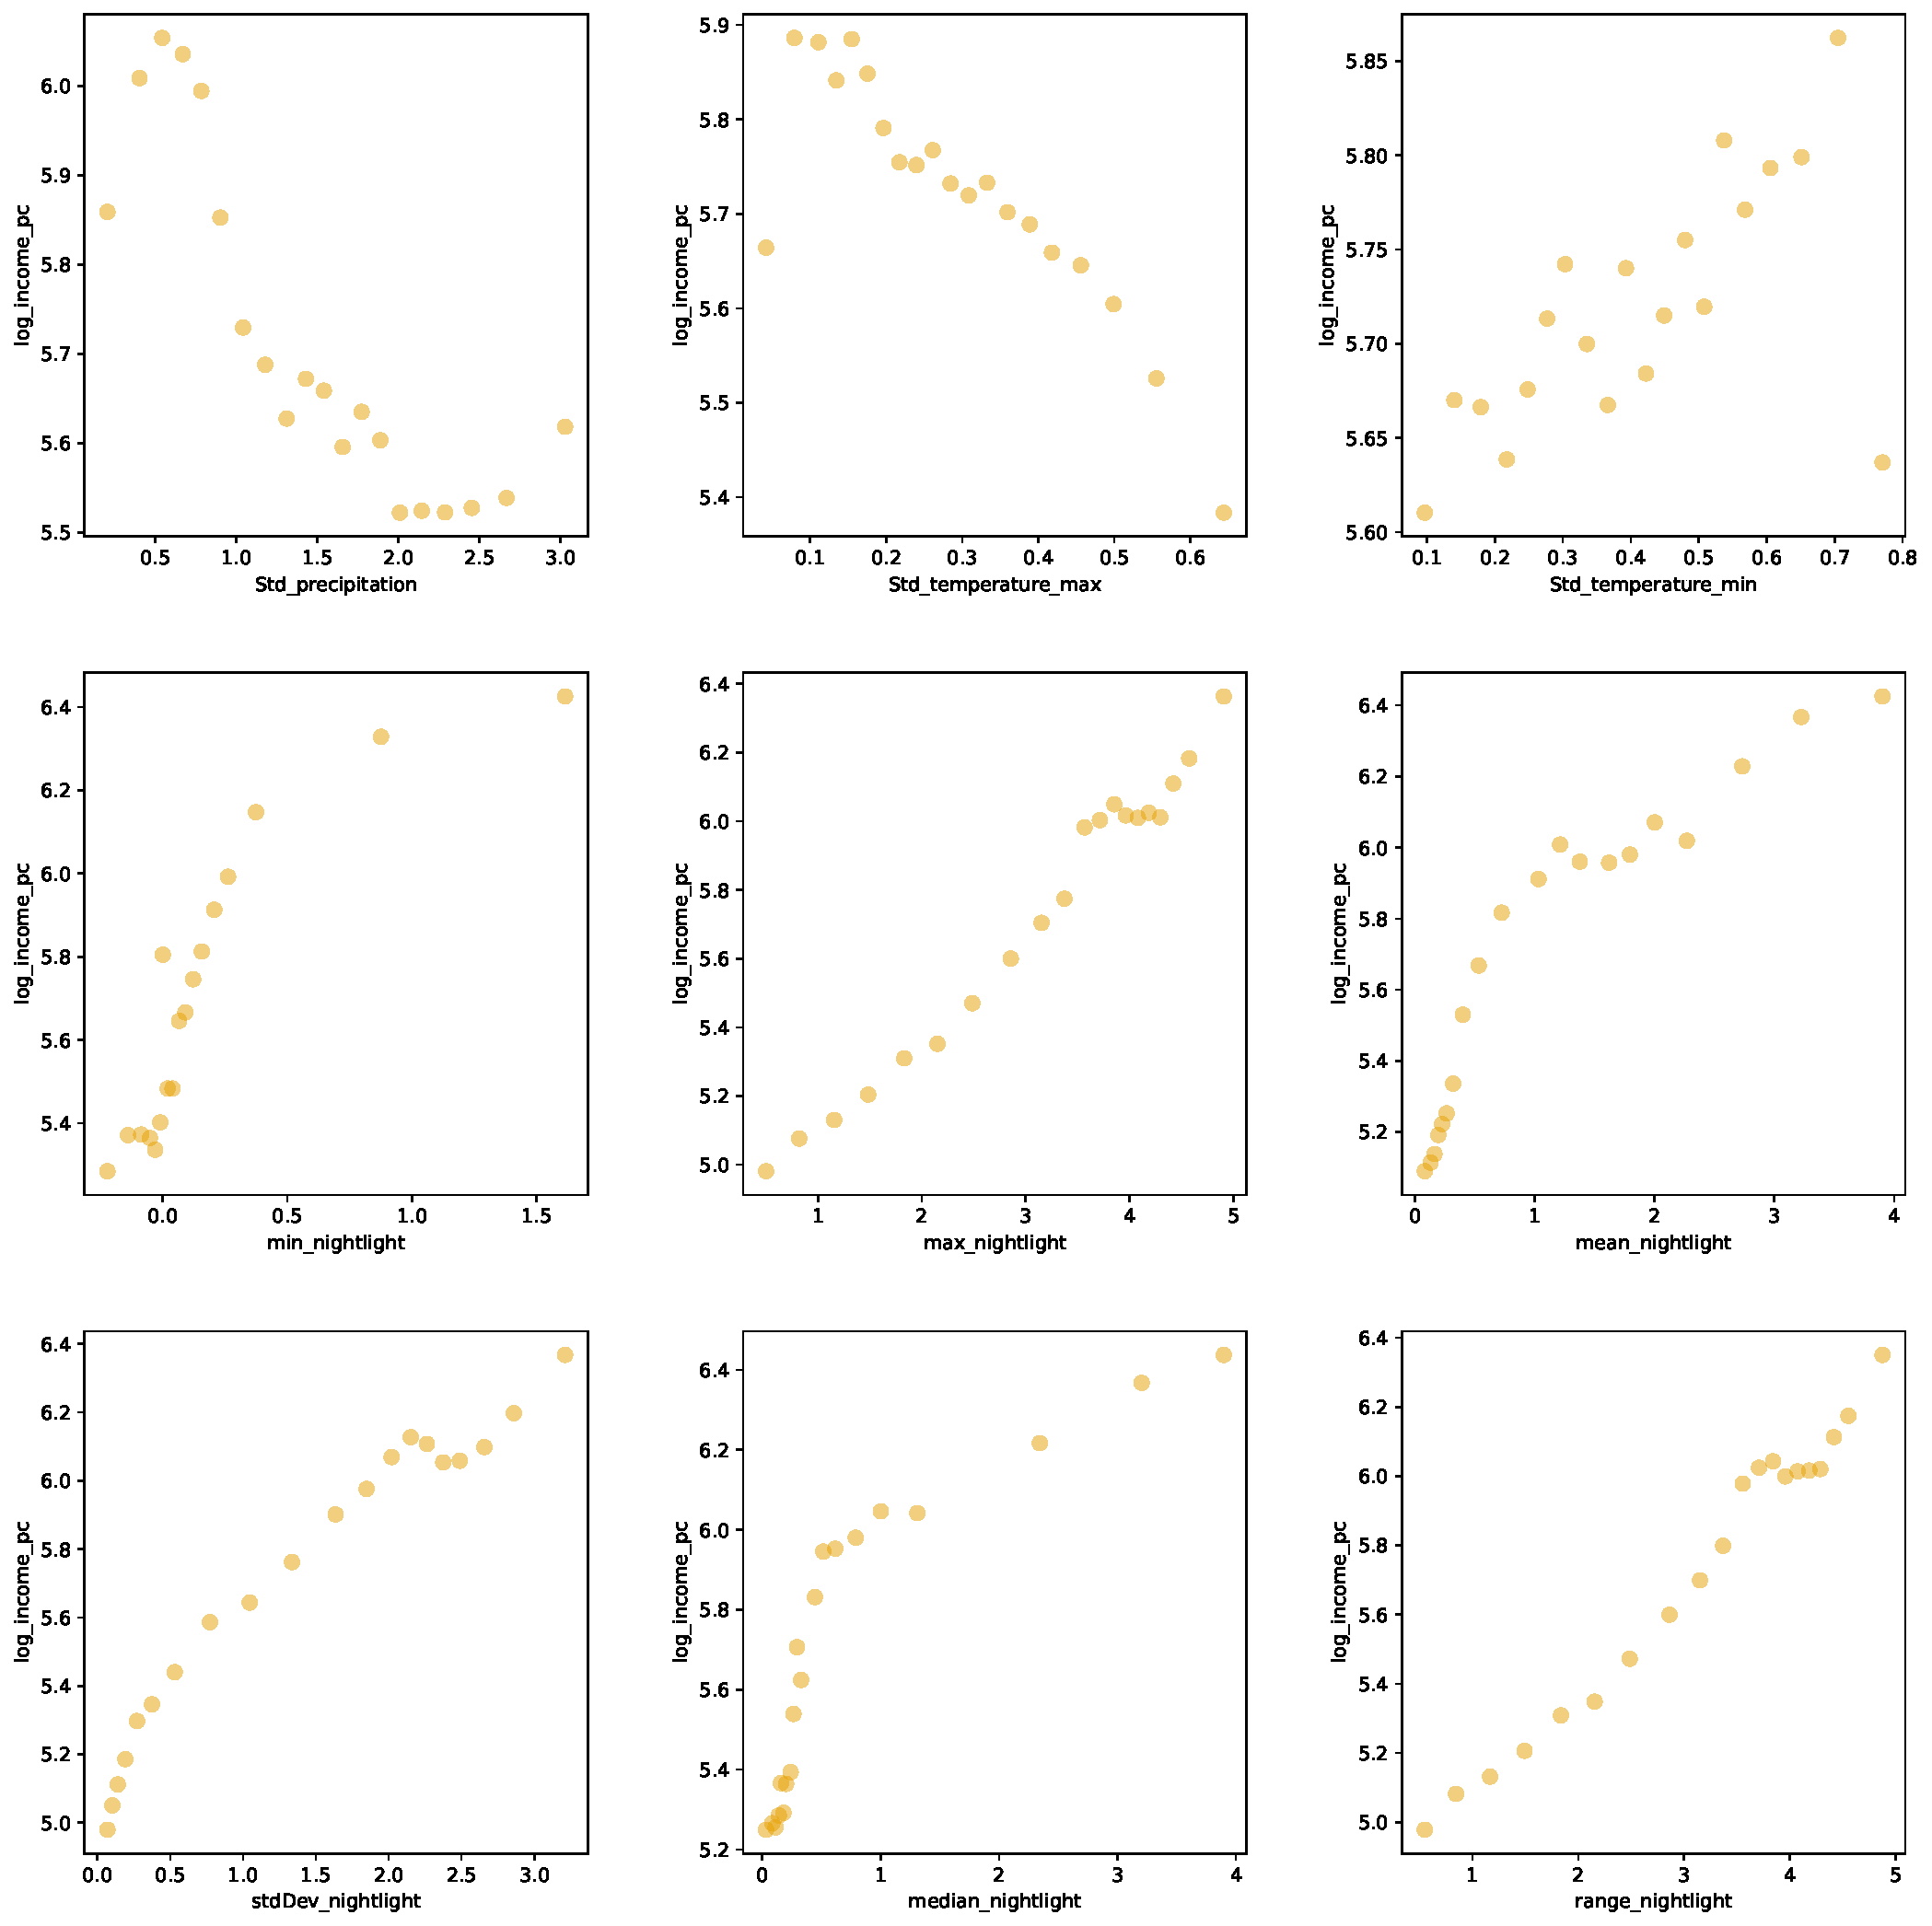
\includegraphics[width=1\textwidth]{../figures/figD_correlation_ml_dataset_weather_variables.pdf}
    \label{fig:enter-label}
\end{figure}


\begin{figure}[H]
    \centering
    \caption{Share of Missing Values}
    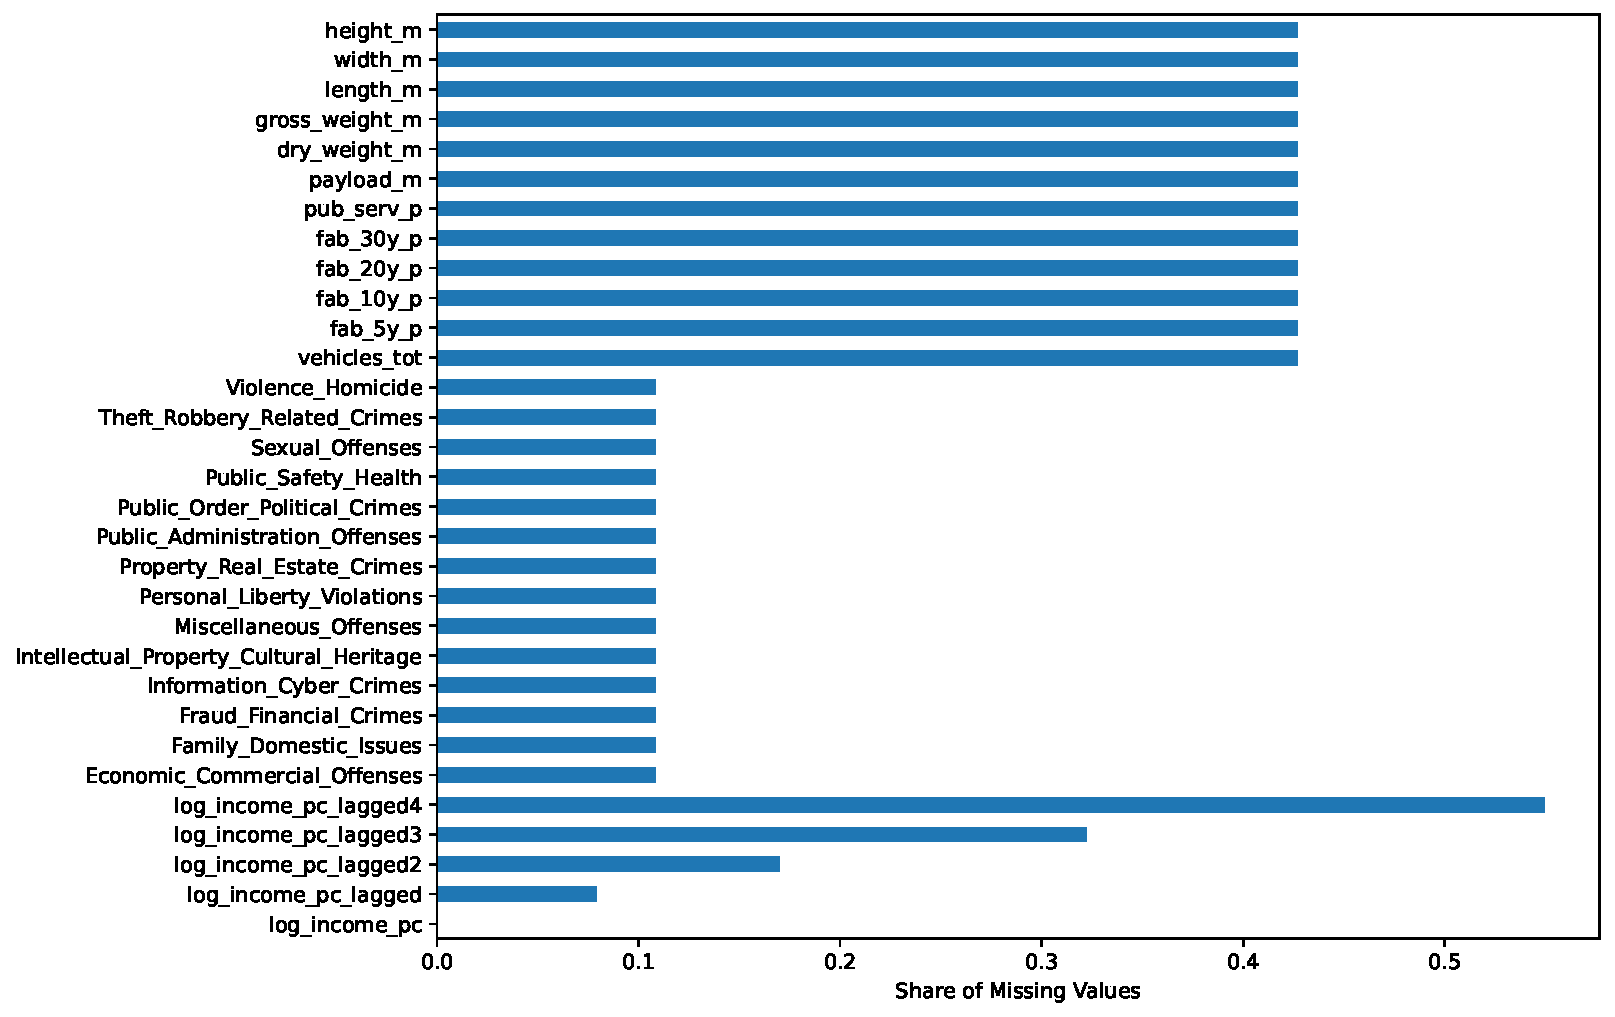
\includegraphics[width=1\textwidth]{../figures/figE_share_of_missings.pdf}
    \label{fig:enter-label}
\end{figure}


\begin{table}[H]
\centering
\caption{Missing lags at CCPP level}
\begin{tabular}{ccccc}
\hline
year  & Lag 1 & Lag 2 & Lag 3 & Lag 4 \\ \hline
2008  & 1     & 1     & 1     & 1     \\
2009  & 0.003 & 1     & 1     & 1     \\
2010  & 0.004 & 0.007 & 1     & 1     \\
2011  & 0.151 & 0.155 & 0.157 & 1     \\
2012  & 0.006 & 0.156 & 0.159 & 0.162 \\
2013  & 0.445 & 0.448 & 0.535 & 0.537 \\
2014  & 0.288 & 0.724 & 0.725 & 0.77  \\
2015  & 0.191 & 0.457 & 0.868 & 0.868 \\
2016  & 0.182 & 0.352 & 0.588 & 0.955 \\
2017  & 0.051 & 0.195 & 0.371 & 0.617 \\
2018  & 0.074 & 0.121 & 0.254 & 0.418 \\
2019  & 0.011 & 0.017 & 0.067 & 0.209 \\
2020  & 0.319 & 0.327 & 0.331 & 0.375 \\ \hline
Total & 0.199 & 0.357 & 0.510 & 0.659 \\ \hline
\end{tabular}
\end{table}